
\subsection{MOST}

\begin{wrapfigure}{r}{0.5\textwidth}
    \begin{tikzpicture}
        \begin{interface}[text width=8cm]{ModuleStateMachine}{0,0}
        \operation{ModuleStateMachine(string moduleName, int EquipletID, int moduleID, bool isActor)}
        \operation{set\_Error() : void}
        \operation[0]{transitionSetup(ActionSever* as) :     void}
        \operation[0]{transitionShutdown(ActionSever* as) : void}
        \operation[0]{transitionStart(ActionSever* as) : void}
        \operation[0]{transitionStp(ActionSever* as) : void}
        \end{interface}
    \end{tikzpicture}
\end{wrapfigure}

MOST is a State Machine for modules.
It is available as interface.
Each module has to implement it. 

The constructor of the ModuleStateMachine asks four parameters. \\
\\
\textbf{\textit{moduleName}} is the name of the module \\
\textbf{\textit{EquipletID}} is the id of the eqiplet the module is attached to \\
\textbf{\textit{moduleID}} is the id of the module itself \\
\textbf{\textit{isActor}} is a boolean indicating of the module is an actor or not. This is used by the set\_Error method \\

\noindent
The MOST implementation consists of four transition methods.
Each method represents a transition.
At the end of a transition the module has to call setSucceeded or setFailed on the given ActionServer.
\\\\
The set\_Error method is used to set the Module on an error mode. In influence of it is an actor module change it the mode. Actor modules have a 'critical error mode' and non-actors have a 'error mode'.

\subsubsection{Implementation}
\begin{figure}[H]
\begin{lstlisting}[language=c++, frame=single, caption=Sample transition]
void ModuleImplementation::transitionSetup(
	rexos_statemachine::TransitionActionServer* as) 
{
	ROS_INFO("Setup transition called");

	//Do groundbreaking initialisation sequence

	if(succeeded)
		as->setSucceeded();
	else
		as->setAborted();
}
\end{lstlisting}
\end{figure}
The transitions must be implemented in the module. Each transition has an TransitionActionServer parameter. This parameter should be used to set the transition succeeded or not by the setSucceeded or setAborted methods. If the transition finished without a call to the TransitionActionServer the State Machine receive an aborted and the change state should be failed.

\subsection{Equiplet}
\subsubsection{Module registration}
The State Machine also takes care of registering itself at the Equiplet. 
When a module starts it waits for an Equiplet with the ID given in the State Machines constructor. 
Then it will send a module registration request. 
The Equiplet will then respond with a success or failure. 
If the registration has failed, the module will shut itself down.

\begin{center}
\begin{sequencediagram}
    \newinst{module}{:Module}
    \newinst{Equiplet}{:Equiplet}
    \begin{call}{module}{ModuleRegistration(moduleName, moduleID)}{Equiplet}{succeed}
    \end{call}
\end{sequencediagram}
\end{center}

\noindent
After registration EST has control over the states and modes of the module.

\subsubsection{EST}
EST is the State Machine in the Equiplet. 
This State Machine has predefined functionality and is implemented for the greatest important parts.

EST controls the state and mode of the Equiplet.
It also manages the state and modes of its attached modules.
EST provides the module registration functionality.
The EST is describe of all state or mode changes from the modules.

\paragraph{Transtions}In the transition the Equiplet control its modules as described in the design. Setup to Setup all modules and Shutdown to Shutdown to all modules. Start and Stop are currently not used, but in the future may be used by a Start to wait on the first module which in Normal and Stop to wait on its last module which in Standby.

\paragraph{Modes}When the module change from mode, the Equiplet inherits the mode. This happened when a module change to error or critical error, so the Equiplet change also its mode. Also when the Equiplet change its mode it the module modes will also changed to this mode. This is an easy and basic implementation of the mode.

\paragraph{Blackboard}The StateBlackboard is the blackboard which contains the State Machine data. In this blackboard two containers has been implemented: EquipletState which contain the equiplet\_id, state and mode of the equiplet and EquipletCommands which provide functionality to change the state and mode of the equiplet. The state can changed by a 'disiredState:int' and the mode can be changed by 'disiredMode:int'. The integer stand for the state or the mode.

\subsection{State machine}
Both EST and MOST are based on the same base State Machine. 

The base State Machine provides a shared interface for controlling the State Machine.
The interface consists of two ROS Actionlib actions for changing the desired state and mode.

\subsubsection{Modes}
The base State Machine also defines some modes. Each essentially allows or disallows certain states and transitions.

When a change mode action is received and the current state is not allowed in the new mode, the State Machine will force the module or Equiplet to go to a allowed state.

\begin{figure}[H]
\caption{
    Example forced state change.
    Module is in normal state.
}
\begin{center}
\begin{sequencediagram}
    \newinst[0]{e}{:Equiplet}
    \newinst[5]{s}{:Statemachine}
    \newinst[1]{m}{:Module}
    \begin{messcall}{e}{changeMode(ERROR)}{s}
    \end{messcall}
    \begin{messcall}{s}{modeChanged(ERROR)}{e}
    \end{messcall}
    \begin{call}{s}{transitionStop}{m}{SUCCESS}
    \end{call}
    \begin{messcall}{s}{stateChanged(STANDBY)}{e}
    \end{messcall}
\end{sequencediagram}
\end{center}
\end{figure}

\subsection{SCADA}
SCADA runs in the same program that is running EST. 
EST provides SCADA with the information it needs. 
SCADA in turn uses EST to send commands to the registered modules.

\begin{figure}[H]
\begin{center}
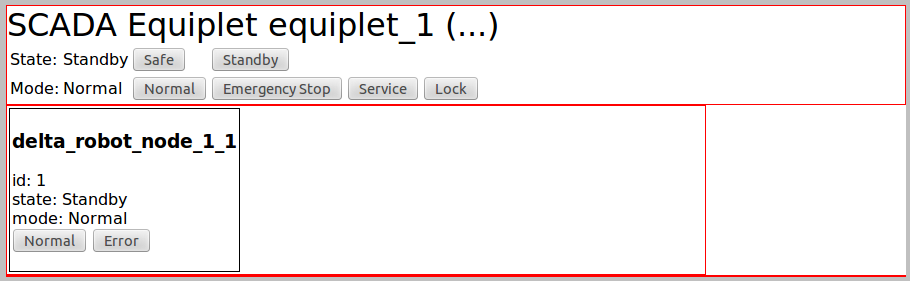
\includegraphics[scale=0.4]{scada.png}
\end{center}
\end{figure}

\section{ROS}
\subsection{Comunication}
ROS is used for inter process calls and communication between nodes.

\subsubsection{Module registration}
When a module is started it tries to register itself in the equiplet node.
The equiplet node only accepts the module when the equiplet is safe.
A module is also rejected if the equiplet already has a module with the same id.

For the registration the equiplet node advertises a service. 
The service is called regiset\_module and is accessible in the equplet nodes namespace. 
(eg. equiplet\_1/register\_module)
The register\_module service has sends the name and the id of the module to the equiplet.

After the module has registered itself the module registry in the equiplet node creates a ModuleProxy. 
the ModuleProxy links to the change\_state and change\_mode actions of the module.

\subsubsection{Change states and modes}
To change the state or mode of a module the equiplet has to search for the module in the ModuleRegistry. 
This registry holds all the registered modules and their proxies. 
Using the proxies the mode and state of the modules can be changed.

The proxies contacts the actionservers in the module which in their turn call their own actioservers for the actual transitions.